\begin{appendices}
\addtocontents{toc}{\protect\setcounter{tocdepth}{0}} % Suppress sub-levels in TOC within appendices


\section{Development setup} \label{app:devsetup}
If working on Windows, the following programs are needed:
\begin{itemize}
    \item CubeMX \ref{app:software:stm32cubemx}
    \item Arm GNU Toolchain (download as zip) \ref{app:software:arm_toolchain}
    \item Visual Studio Code \ref{app:software:vsc}
    \item OpenOCD \ref{app:software:openocd}
    \item Git (download as zip) \ref{app:software:git}
\end{itemize}

And the following binaries:
\begin{itemize}
    \item Make for Windows with dependencies \ref{app:software:make}
\end{itemize}

\begin{enumerate}
    \item Download all of the files, install VSCode and CubeMX and unpack the rest to a folder of your choice.
    \item Setup a new project in CubeMX, and change the toolchain under the project manager to \lstinline[style=bash]{Makefile}
    \item Add paths to system environment variables.
    \begin{enumerate}
        \item Add new variable with name \lstinline[style=bash]{ARMGCC\_DIR} with value \lstinline[style=bash]{<your path>\arm-gnu-toolchain-<version>.Rel1-mingw-w64-i686-arm-none-eabi\bin}
        \item Edit path variable and add:
        \begin{enumerate}
            \item \lstinline[style=bash]{\%ARMGCC\_DIR\%}
            \item \lstinline[style=bash]{<your path>\make-<version>\bin}
            \item \lstinline[style=bash]{<your path>\OpenOCD-<version>\bin}
            \item \lstinline[style=bash]{<your path>\git\bin}
            \item \lstinline[style=bash]{<your path>\git\usr\bin}
        \end{enumerate}
    \end{enumerate}
    \item Open a new terminal and test that the environment variables are set correctly by running \lstinline[style=bash]{make --version}, \lstinline[style=bash]{openocd --version}, \lstinline[style=bash]{git --version} and \lstinline[style=bash]{arm-none-eabi --version}. If every command returns a version number, your environment variables have been updated correctly.
    \item Test that you can compile, by going into your newly created project directory and running the command \lstinline[style=bash]{make}.
    If no error appears, a hex and bin-file are created inside the newly created folder: \lstinline[style=bash]{...\build\<project-name>.hex}.
    \item Open the newly created \lstinline[style=bash]{Makefile} and add the following:
    \begin{lstlisting}[style=bash]
        #######################################
        # openocd
        #######################################
        flash: all
       openocd -f interface/stlink.cfg -f target/@board version@.cfg -c "program $(BUILD_DIR)/$(TARGET).elf verify reset exit"
    \end{lstlisting}
    where the corresponding cfg file for your board, should be found in: \\ 
    \lstinline[style=bash]{<your path>\OpenOCD-<version>\share\openocd\scripts\target}
    \item You should now be able to flash the board by running the command \lstinline[style=bash]{make flash} in a terminal in the project directory.
 \end{enumerate}



Another way to set this up on Windows is to use \ac{WSL}.

%\textcolor{red}{Hvis man gør dette, skal man også bruge VSCode gennem WSL. Det har vi ikke prøvet endnu, men det burde jo egentlig virke}

If working on a Windows machine, open PowerShell and run the following to install \ac{WSL} \sbref{app:software:wsl}.
\begin{lstlisting}[style=bash]
sudo apt update && sudo apt upgrade
wsl --install
\end{lstlisting}
The machine is now set up like a Linux machine and can perform alike.

To fetch, compile and run the firmware code in the GitHub repository, the user needs to install Git \sbref{app:software:git}, GNU Make \sbref{app:software:make}, ARM GNU Toolchain \sbref{app:software:arm_toolchain}, and OpenOCD \sbref{app:software:openocd}.
\begin{lstlisting}[style=bash]
sudo apt install git make gcc-arm-none-eabi openocd
\end{lstlisting}

When installed, the GitHub repository \sbref{app:code} can be cloned\footnote{Cloning a repository: \url{https://docs.github.com/en/repositories/creating-and-managing-repositories/cloning-a-repository}} to a desired directory, and the development can start using an \ac{IDE}.

\subsection{Visual Studio Code integration}
The preferred \ac{IDE} used in this project is Visual Studio Code \sbref{app:software:vsc}. Open the newly cloned repository and, if in Windows, run in the terminal \lstinline[style=bash]{wsl} to start performing like a Linux machine.

The compiling of the project is based on a simple makefile and can be compiled with:
\begin{lstlisting}[style=bash]
make
make -f CustomeNameMakefile     # used for custom names
\end{lstlisting}
If no error appears, a hex-file is created inside the newly created folder (\lstinline[style=bash]{build\VSC_win.hex}), and can be flashed to the STM32 chip with \lstinline[style=bash]{make flash}.

For debugging, install Cortex-Debug \sbref{app:software:cortex_debug} in the Extension Marketplace.

Create a new folder called ".vscode" for personal setup of the debugging and running of the code and add two files from appendix \sbref{app:software:c_cpp_properties} and \sbref{app:software:launch}.

\section{Code} \label{app:code}
All code is available on GitHub at \url{https://github.com/MagnusErler/WiFiLocationTracker}.\\
Update firmware: \url{https://github.com/Lora-net/lr1110_updater_tool/wiki}\\
\url{https://github.com/Lora-net/SWTL001/wiki}

\section{Essential hardware} \label{app:hardware}
\begin{enumerate}
    \item LR1110 : \url{https://www.semtech.com/products/wireless-rf/lora-edge/lr1110} \label{app:hardware:lr1110}
    \item STM32L476RG : \url{https://www.st.com/en/microcontrollers-microprocessors/stm32l476rg.html} \label{app:hardware:stm32l476rg}
    \item NT2016SA 32MHz END4263A : \url{https://www.digikey.dk/en/products/detail/ndk-america-inc/NT2016SA-32M-END4263A/8275433} \label{app:hardware:tcxo}
    \item LIS2DE12 : \url{https://www.st.com/resource/en/datasheet/lis2de12.pdf} \label{app:hardware:lis2de12}
    \item BU52077GWZ : \url{https://fscdn.rohm.com/en/products/databook/datasheet/ic/sensor/hall/bu52077gwz-e.pdf} \label{app:hardware:BU52077GWZ}
    \item XC6220B331MR : \url{https://product.torexsemi.com/system/files/series/xc6220.pdf} \label{app:hardware:XC6220}
    \item BGA524N6E6327 : \url{https://www.infineon.com/dgdl/Infineon-BGA524N6-DataSheet-v03_05-EN.pdf?fileId=db3a304344e406b50144e44dfad302b9} \label{app:hardware:bga524n6e6327}
\end{enumerate}

\section{Essential software}  \label{app:software}
\begin{enumerate}
    \item Visual Studio Code : \url{https://code.visualstudio.com/} \label{app:software:vsc}
    \item STM32CubeMX : \url{https://www.st.com/content/st_com/en/stm32cubemx.html} \label{app:software:stm32cubemx}
    \item Git : \url{https://git-scm.com/} \label{app:software:git}
    \item GNU Make : \url{https://gnuwin32.sourceforge.net/packages/make.htm} \label{app:software:make}
    \item ARM GNU Toolchain : \url{https://developer.arm.com/downloads/-/gnu-rm}
    https://developer.arm.com/downloads/-/gnu-rm
    \label{app:software:arm_toolchain}
    \item OpenOCD : \url{https://gnutoolchains.com/arm-eabi/openocd/} \label{app:software:openocd}
    \item Cortex-Debug : \url{https://marketplace.visualstudio.com/items?itemName=marus25.cortex-debug} \label{app:software:cortex_debug}
    \item WSL : \url{https://learn.microsoft.com/en-us/windows/wsl/install} \label{app:software:wsl}
    \item AppCAD : \url{https://www.broadcom.com/info/wireless/appcad} \label{app:software:appcad}
\end{enumerate}

And the following binaries:
- Make for Windows with dependencies \url{https://gnuwin32.sourceforge.net/packages/make.htm} 

\section{Windows and Linux setup}
\subsection*{\lstinline[style=bash]{c_cpp_properties.json}} \label{app:software:c_cpp_properties}
\begin{lstlisting}[language=json]
{
    "configurations": [
        {
            "name": "STM32L476RG",
            "includePath": [
                "${workspaceFolder}/**",
                "${workspaceFolder}/Src/radio/lr1110_modem/src"
            ],
            "defines": [
                "USE_HAL_DRIVER",
                "STM32L476xx"
            ],
            "configurationProvider": "ms-vscode.makefile-tools",
            "compilerPath": "C:/Program Files (x86)/Microsoft Visual Studio/2022/BuildTools/VC/Tools/MSVC/14.38.33130/bin/Hostx64/x64/cl.exe", // Use "which arm-none-eabi-gcc" to get the location of the compiler in linux
            "compilerArgs": [
                "-mcpu=cortex-m4",
                "-mthumb"
            ],
            "cStandard": "c11",
            "cppStandard": "c++17"
        }
    ],
    "version": 4
}
\end{lstlisting}

\subsection*{\lstinline[style=bash]{launch.json}} \label{app:software:launch}
\begin{lstlisting}[language=json]
{
    "version": "0.2.0",
    "configurations": [
        {
            "name": "Cortex Debug",
            "cwd": "${workspaceFolder}",
            "executable": "./build/VSC_win.elf",
            "request": "launch",
            "type": "cortex-debug",
            "runToEntryPoint": "main",
            "servertype": "openocd",
            "device": "STM32L476RG",
            "configFiles": [
                "interface/stlink.cfg",
                "target/stm32l4x.cfg"
            ]
        }
    ]
}
\end{lstlisting}

\section{PCB}

\subsection{BOM} \label{app:BOM}

\begin{footnotesize}
\begin{longtable}{llllll}
    \caption{BOM of the tracker.} \\
    \toprule
    Name & Designator & Footprint & Manufacturer Part & Manufacturer & Price [\$] \\
    \midrule
    \endfirsthead
    
    \multicolumn{6}{c}{\normalsize{\tablename\ \thetable{} BOM.}} \\
    \toprule
    Name & Designator & Footprint & Manufacturer Part & Manufacturer & Price [\$] \\
    \midrule
    \endhead
    
    %\bottomrule
    %\multicolumn{6}{r}{{Continued on next page}} \\
    \endfoot
    
    %\bottomrule
    \endlastfoot

    \multicolumn{6}{c}{\cellcolor[HTML]{EFEFEF}Chips} \\
    STM32L476 & U1 & LQFP-64 & STM32L476RET6 & ST & 2.924 \label{bom:stm32l476} \\
    LR1110 & U2 & QFN-50 & LR1110IMLTRT & Semtech & 10.54 \label{bom:lr1110}\\
    SKY13588-460LF & U3 & QFN-12 & SKY13588-460LF & SKYWORKS & 2.254 \\
    BGA524N6E6327 & U4 & TSNP-6 & BGA524N6E6327 & Infineon & 0.286 \label{bom:bga524n6e6327}\\
    XC6220B331MR & U5 & SOT23-5 & XC6220B331MR & TECH PUBLIC & 0.179 \label{bom:xc6220} \\
    LIS2DE12TR & U6 & LGA-12 & LIS2DE12TR & ST & 0.469 \label{bom:lis2de12}\\
    BU52077GWZ-E2 & U7 & BGA-4 & BU52077GWZ-E2 & ROHM & 0.177 \label{bom:bu52077gwz}\\

    \multicolumn{6}{c}{\cellcolor[HTML]{EFEFEF}Resistors} \\
    \SI{220}{\ohm} & R3 & R0402 & 0402WGF2200TCE & UNI-ROYAL & 0.001 \\
    \SI{10}{\kilo\ohm} & R7 & R0402 & 0402WGF1002TCE & UNI-ROYAL & 0.001 \\
    \SI{200}{\ohm} & R33 & R0603 & 0603WAF2000T5E & UNI-ROYAL & 0.001 \\

    \multicolumn{6}{c}{\cellcolor[HTML]{EFEFEF}Capacitors} \\
    \SI{100}{\nano\farad} & C1 & C0402 & CL05B104KO5NNNC & SAMSUNG & 0.001 \\
    \SI{47}{\pico\farad} & C2 & C0402 & 0402CG470J500NT & FH & 0.001 \\
    \SI{470}{\nano\farad} & C3 & C0603 & CL10B474KA8NNNC & SAMSUNG & 0.007 \\
    \SI{100}{\nano\farad} & C4 & C0402 & CL05B104KO5NNNC & SAMSUNG & 0.001 \\
    \SI{2.2}{\nano\farad} & C5 & C0603 & 0603B222K500NT & FH & 0.002 \\
    \SI{47}{\pico\farad} & C6 & C0402 & 0402CG470J500NT & FH & 0.001 \\
    \SI{47}{\pico\farad} & C7 & C0402 & 0402CG470J500NT & FH & 0.001 \\
    \SI{1}{\pico\farad} (1.2p) & C8 & C0402 & 0402CG1R0C500NT & FH & 0.001 \\
    \SI{10}{\pico\farad} (6.8p) & C9 & C0402 & CL05C100JB5NNNC & SAMSUNG & 0.005 \\
    \SI{47}{\pico\farad} & C10 & C0402 & 0402CG470J500NT & FH & 0.001 \\
    \SI{1}{\pico\farad} (1.8p) & C12 & C0402 & 0402CG1R0C500NT & FH & 0.001 \\
    \SI{1}{\pico\farad} (3.0p) & C13 & C0402 & 0402CG1R0C500NT & FH & 0.001 \\
    \SI{10}{\pico\farad} (6.8p) & C14 & C0402 & CL05C100JB5NNNC & SAMSUNG & 0.005 \\
    \SI{47}{\pico\farad} & C15 & C0402 & 0402CG470J500NT & FH & 0.001 \\
    \SI{1}{\pico\farad} (1.5p) & C17 & C0402 & 0402CG1R0C500NT & FH & 0.001 \\
    \SI{1}{\pico\farad} (1.2p) & C18 & C0402 & 0402CG1R0C500NT & FH & 0.001 \\
    \SI{1}{\pico\farad} (1.5p) & C19 & C0402 & 0402CG1R0C500NT & FH & 0.001 \\
    \SI{47}{\pico\farad} & C21 & C0402 & 0402CG470J500NT & FH & 0.001 \\
    \SI{1}{\pico\farad} & C22 & C0402 & 0402CG1R0C500NT & FH & 0.001 \\
    \SI{1}{\pico\farad} (1.5p) & C23 & C0402 & 0402CG1R0C500NT & FH & 0.001 \\
    \SI{1}{\pico\farad} (0.5p) & C24 & C0402 & 0402CG1R0C500NT & FH & 0.001 \\
    \SI{12}{\pico\farad} & C25 & C0402 & 0402CG120J500NT & FH & 0.001 \\
    \SI{1}{\pico\farad} (0.5p) & C26 & C0402 & 0402CG1R0C500NT & FH & 0.001 \\
    \SI{1}{\pico\farad} (1.3p) & C27 & C0402 & 0402CG1R0C500NT & FH & 0.001 \\
    \SI{1}{\pico\farad} (1.6p) & C28 & C0402 & 0402CG1R0C500NT & FH & 0.001 \\
    \SI{33}{\pico\farad} & C29 & C0402 & 0402CG330J500NT & FH & 0.001 \\
    \SI{1}{\pico\farad} (0.7p) & C30 & C0402 & 0402CG1R0C500NT & FH & 0.001 \\
    \SI{1}{\pico\farad} (3.3p) & C31 & C0402 & 0402CG1R0C500NT & FH & 0.001 \\
    \SI{1}{\pico\farad} (3.3p) & C32 & C0402 & 0402CG1R0C500NT & FH & 0.001 \\
    \SI{100}{\nano\farad} & C33 & C0402 & CL05B104KO5NNNC & SAMSUNG & 0.001 \\
    \SI{1}{\micro\farad} & C34 & C0402 & CL05A105KA5NQNC & SAMSUNG & 0.004 \\
    \SI{100}{\nano\farad} & C35 & C0402 & CL05B104KO5NNNC & SAMSUNG & 0.001 \\
    \SI{100}{\nano\farad} & C36 & C0402 & CL05B104KO5NNNC & SAMSUNG & 0.001 \\
    \SI{100}{\nano\farad} & C37 & C0402 & CL05B104KO5NNNC & SAMSUNG & 0.001 \\
    \SI{10}{\micro\farad} & C38 & C0603 & CL10A106KP8NNNC & SAMSUNG & 0.005 \\
    \SI{1}{\nano\farad} & C39 & C0402 & 0402B102K500NT & FH & 0.001 \\
    \SI{1}{\micro\farad} & C40 & C0402 & CL05A105KA5NQNC & SAMSUNG & 0.004 \\
    \SI{10}{\nano\farad} & C41 & C0402 & CL05B103KB5NNNC & SAMSUNG & 0.001 \\
    \SI{4.7}{\micro\farad} & C42 & C0402 & CL05A475MP5NRNC & SAMSUNG & 0.005 \\
    \SI{1}{\nano\farad} & C43 & C0402 & 0402B102K500NT & FH & 0.001 \\
    \SI{1}{\micro\farad} & C44 & C0402 & CL05A105KA5NQNC & SAMSUNG & 0.004 \\
    \SI{1}{\nano\farad} & C45 & C0402 & 0402B102K500NT & FH & 0.001 \\
    \SI{1}{\nano\farad} & C46 & C0402 & 0402B102K500NT & FH & 0.001 \\
    \SI{100}{\nano\farad} & C47 & C0402 & CL05B104KO5NNNC & SAMSUNG & 0.001 \\
    \SI{10}{\micro\farad} & C48 & C0402 & CL05A106MQ5NUNC & SAMSUNG & 0.005 \\
    \SI{100}{\nano\farad} & C49 & C0402 & CL05B104KO5NNNC & SAMSUNG & 0.001 \\
    \SI{10}{\pico\farad} & C50 & C0402 & CL05C100JB5NNNC & SAMSUNG & 0.005 \\
    \SI{1}{\pico\farad} (1.8p) & C51 & C0402 & 0402CG1R0C500NT & FH & 0.001 \\
    \SI{1}{\pico\farad} (0.5p) & C52 & C0402 & 0402CG1R0C500NT & FH & 0.001 \\
    \SI{1}{\nano\farad} & C54 & C0402 & 0402B102K500NT & FH & 0.001 \\
    \SI{470}{\pico\farad} & C55 & C0603 & 0603B471K500NT & FH & 0.002 \\
    \SI{1}{\pico\farad} (0.5p) & C56 & C0402 & 0402CG1R0C500NT & FH & 0.001 \\
    \SI{1}{\pico\farad} (1.8p) & C57 & C0402 & 0402CG1R0C500NT & FH & 0.001 \\
    \SI{1}{\nano\farad} & C58 & C0402 & 0402B102K500NT & FH & 0.001 \\
    \SI{100}{\nano\farad} & C81 & C0402 & CL05B104KO5NNNC & SAMSUNG & 0.001 \\
    \SI{4.7}{\micro\farad} & C82 & C0402 & CL05A475MP5NRNC & SAMSUNG & 0.005 \\
    \SI{100}{\nano\farad} & C101 & C0402 & CL05B104KO5NNNC & SAMSUNG & 0.001 \\
    \SI{100}{\nano\farad} & C103 & C0402 & CL05B104KO5NNNC & SAMSUNG & 0.001 \\
    \SI{1}{\micro\farad} & C104 & C0402 & CL05A105KA5NQNC & SAMSUNG & 0.004 \\
    \SI{1}{\micro\farad} & C105 & C0402 & CL05A105KA5NQNC & SAMSUNG & 0.004 \\
    \SI{1}{\micro\farad} & C106 & C0402 & CL05A105KA5NQNC & SAMSUNG & 0.004 \\
    \SI{10}{\ohm} & FB1 & L0402 & CBW100505U100T & FH & 0.004 \\

    \multicolumn{6}{c}{\cellcolor[HTML]{EFEFEF}Inductors \& Ferrites} \\
    \SI{600}{\ohm} & L1 & L0603 & GZ1608D601TF & Sunlord & 0.004 \\
    \SI{10}{\micro\henry} (15u) & L2 & L0805 & SDFL2012S100KTF & Sunlord & 0.016 \\
    \SI{10}{\nano\henry} (47n) & L3 & L0402 & SDCL1005C10NJTDF & Sunlord & 0.003 \\
    \SI{10}{\nano\henry} (47n) & L4 & L0402 & SDCL1005C10NJTDF & Sunlord & 0.003 \\
    \SI{10}{\nano\henry} (3.3n) & L5 & L0402 & SDCL1005C10NJTDF & Sunlord & 0.003 \\
    \SI{10}{\nano\henry} (8.2n) & L6 & L0402 & SDCL1005C10NJTDF & Sunlord & 0.003 \\
    \SI{10}{\nano\henry} (2.7n) & L7 & L0402 & SDCL1005C10NJTDF & Sunlord & 0.003 \\
    \SI{10}{\nano\henry} (6.8n) & L8 & L0402 & SDCL1005C10NJTDF & Sunlord & 0.003 \\
    \SI{10}{\nano\henry} (22n) & L9 & L0402 & SDCL1005C10NJTDF & Sunlord & 0.003 \\
    \SI{10}{\nano\henry} (47n) & L10 & L0402 & SDCL1005C10NJTDF & Sunlord & 0.003 \\
    \SI{10}{\nano\henry} (9.5n) & L11 & L0402 & SDCL1005C10NJTDF & Sunlord & 0.003 \\
    \SI{10}{\nano\henry} (33n) & L12 & L0402 & SDCL1005C10NJTDF & Sunlord & 0.003 \\
    \SI{10}{\nano\henry} (8.5n) & L13 & L0402 & SDCL1005C10NJTDF & Sunlord & 0.003 \\
    \SI{10}{\nano\henry} (8.2n) & L14 & L0402 & SDCL1005C10NJTDF & Sunlord & 0.003 \\
    \SI{10}{\nano\henry} (3.6n) & L15 & L0402 & SDCL1005C10NJTDF & Sunlord & 0.003 \\
    \SI{10}{\nano\henry} (9.1n) & L17 & L0402 & SDCL1005C10NJTDF & Sunlord & 0.003 \\
    \SI{10}{\nano\henry} (3.6n) & L20 & L0402 & SDCL1005C10NJTDF & Sunlord & 0.003 \\
    
    \multicolumn{6}{c}{\cellcolor[HTML]{EFEFEF}Crystals \& \ac{TCXO}} \\
    \SI{32}{\mega\hertz} & X1 & OSC-4 & 1XXD32000MBA & KDS & 0.782 \\
    \SI{32.768}{\kilo\hertz} & X2 & FC-135R & Q13FC13500004 & EPSON & 0.185 \\
    \SI{32.768}{\kilo\hertz} & X3 & FC-135R & Q13FC13500004 & EPSON & 0.185 \\

    \multicolumn{6}{c}{\cellcolor[HTML]{EFEFEF}Connectors} \\
    Wi-Fi U.FL & RF1 & FRF05002 & U.FL-R-SMT-1(80) & HRS & 0.080 \\
    GNSS U.FL & RF2 & FRF05002 & U.FL-R-SMT-1(80) & HRS & 0.080 \\
    LoRa U.FL & RF3 & FRF05002 & U.FL-R-SMT-1(80) & HRS & 0.080 \\

    \midrule
    \multicolumn{4}{l}{\textbf{Total}} & \multicolumn{2}{l}{\hfill\hfill\hfill\hfill\hfill$\$ \ 18.056$} \\
    \bottomrule
    \bottomrule
\end{longtable}
\end{footnotesize}

\begin{landscape}
    \subsection{Wiring diagram} \label{app:wiringDiagram}
    \begin{figure}[H]  
        \centering
        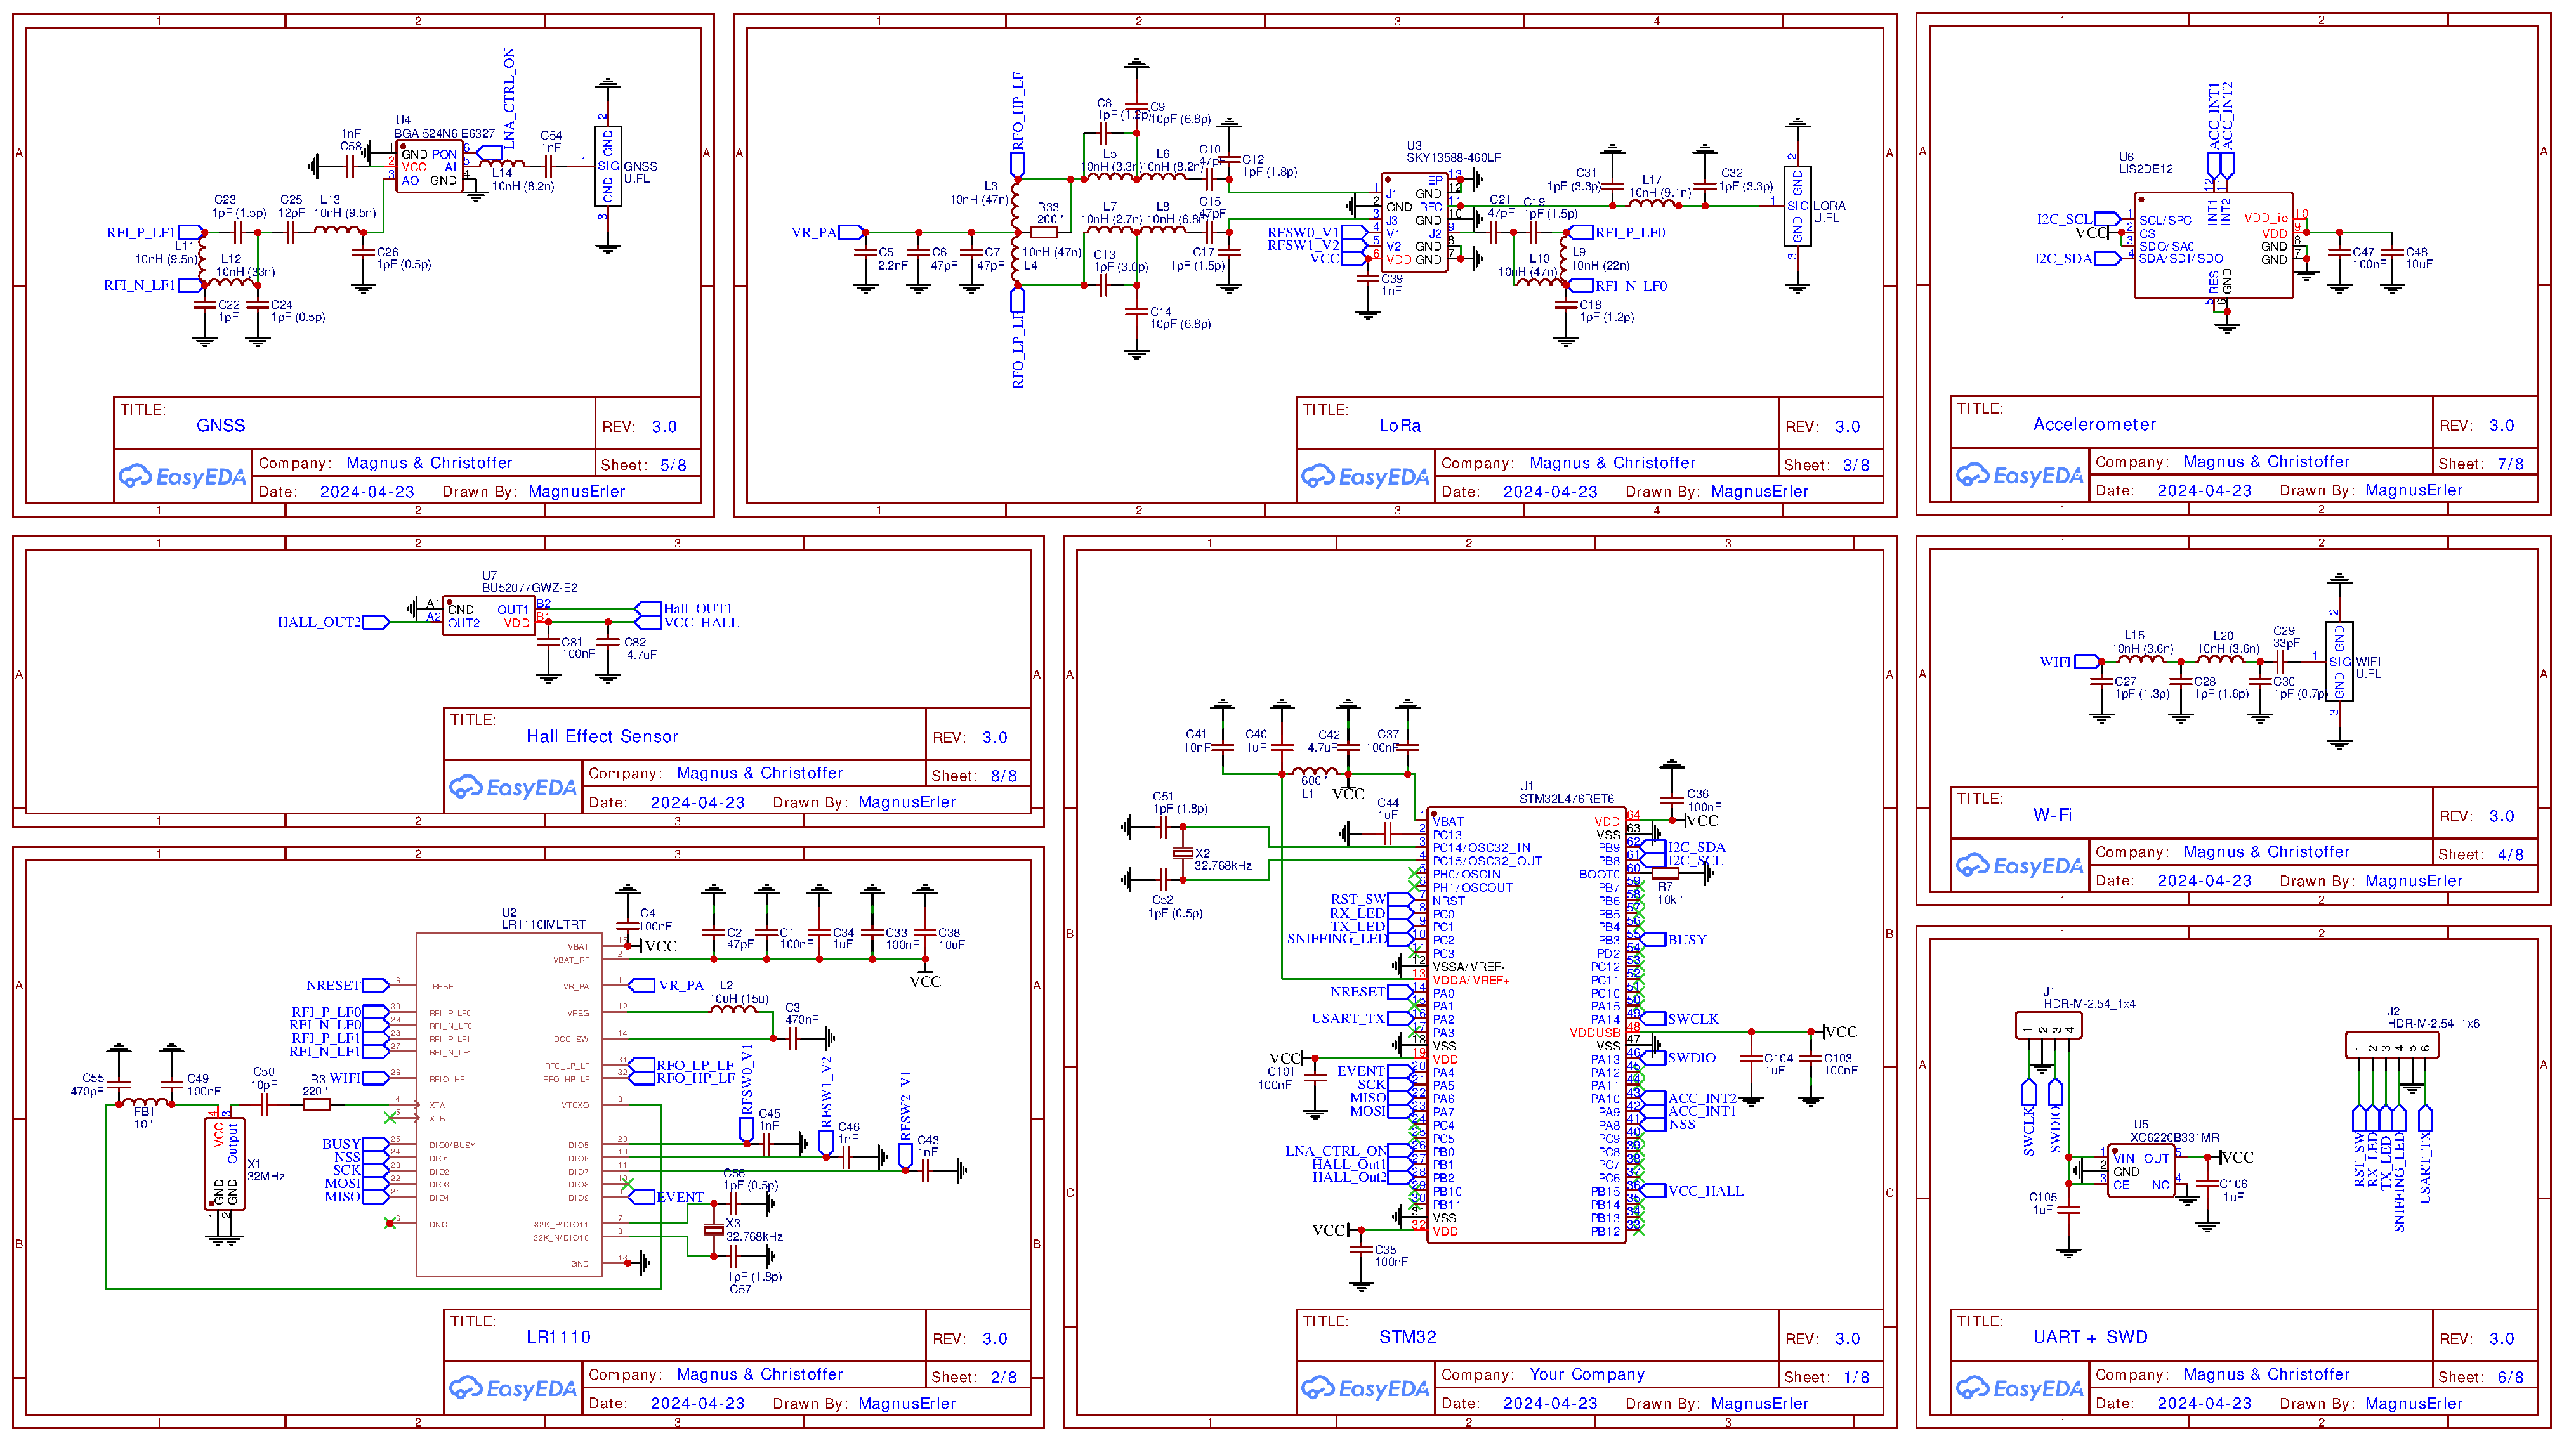
\includegraphics[width=1.38\textwidth]{figures/Schematic.pdf}
        \caption{Overview of the final schematic.}
    \end{figure}
\end{landscape}

\begin{landscape}
    \subsection{PCB} \label{app:PCB}
    \begin{figure}[H]  
        \centering
        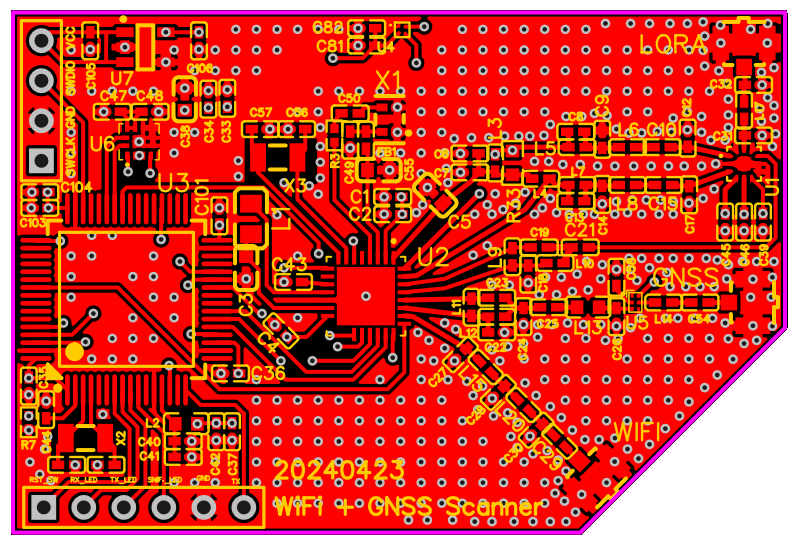
\includegraphics[width=1\textwidth]{figures/PCB_v3.png}
        \caption{Overview of the final PCB.}
    \end{figure}
\end{landscape}

\begin{landscape}
    \subsection{3D view} \label{app:3DView}
    \begin{figure}[H]  
        \centering
        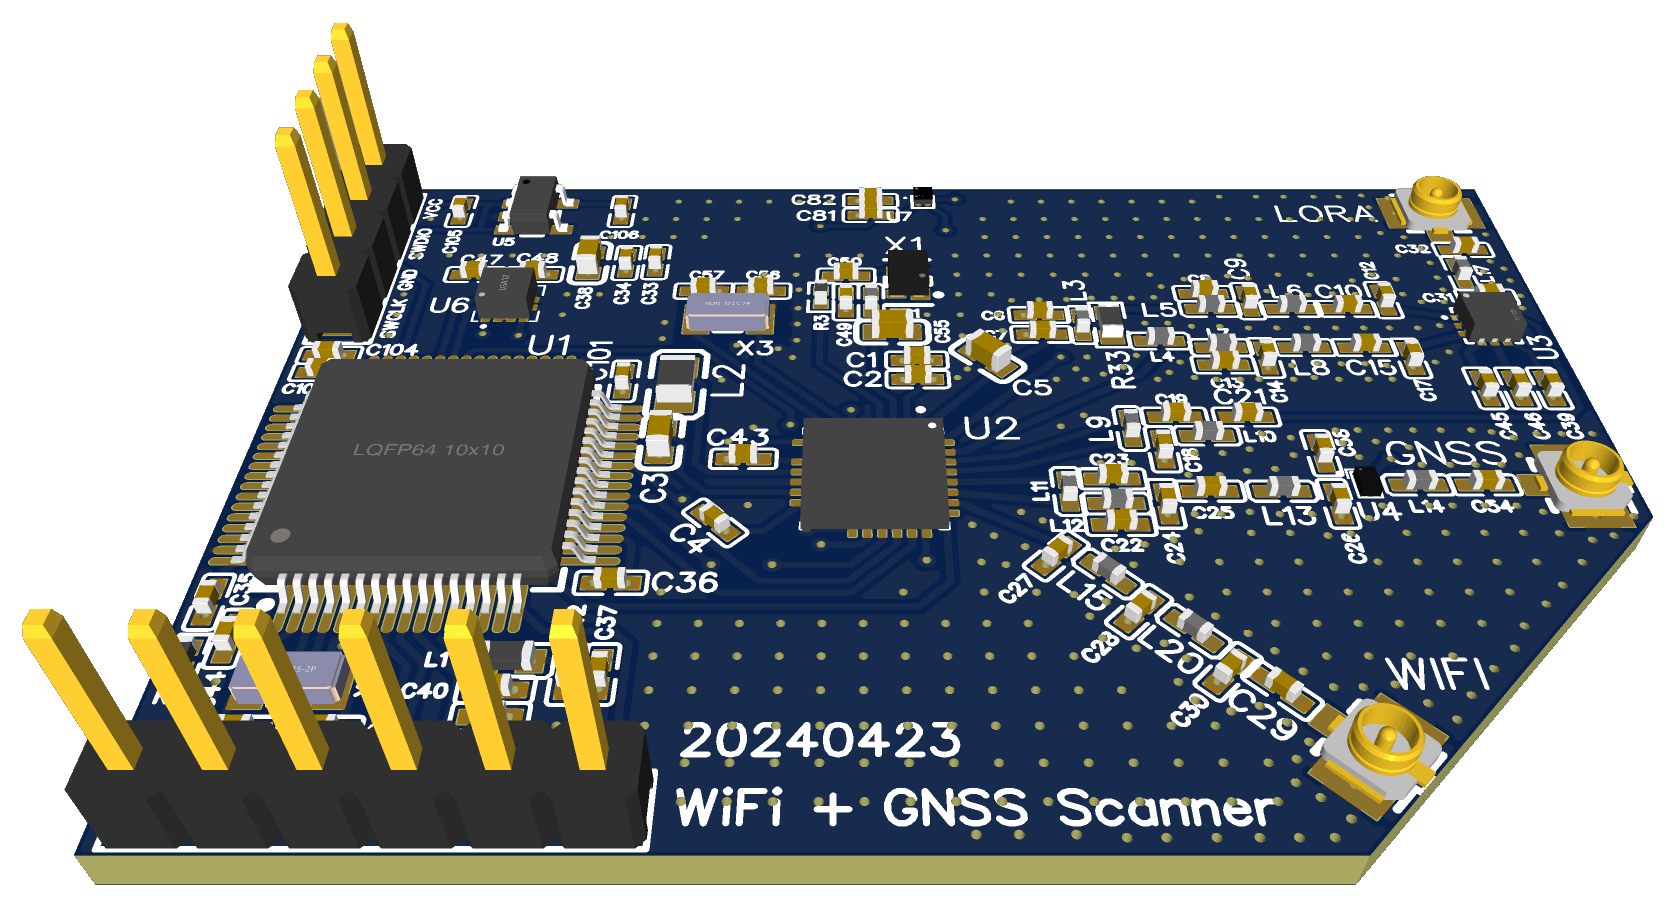
\includegraphics[width=1.38\textwidth]{figures/PCB_v3_3D.png}
        \caption{3D view of the final PCB.}
    \end{figure}
\end{landscape}

\end{appendices}